\FloatBarrier
\begin{figure}[!h]
\centering
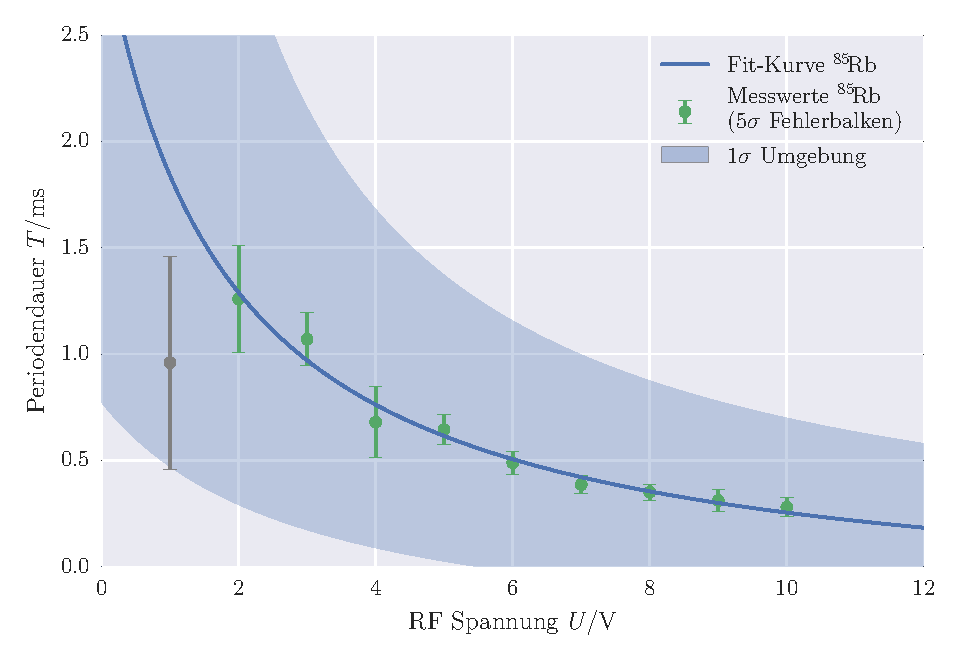
\includegraphics[scale=.85]{../Grafiken/Transienteneffekt_ausgelassen_Rubidium_85.pdf}
\caption{In Abhängigkeit der RF-Spannung dargestellte Periodendauern der Relaxation
	für das Isotop ${}^{85}\!$Rb. Die Fehlerbalken der Messwerte wurden verfünffacht, 
	um sichtbar zu sein. Zusätzlich ist die hyperbolische Ausgleichskurve für die Messwerte
	dargestellt, wobei der grau dargestellte Messwert ausgelassen wurde. 
	\label{fig:transienteneffekt_ausgelassen_rubidium_85}}
\end{figure}
\FloatBarrier